\section{Materials and Methods}\label{materials-and-methods}

This section presents simulation-based experimental methodology testing whether dynamic personality modeling, theoretically grounded regulation, and validated evaluation produce measurable improvements in conversational personalization. We employ a $2 \times 2$ factorial design comparing personality-adaptive (regulated) agents against non-adaptive (baseline) agents across two extreme personality profiles.

\subsection{Overview and Research Objectives}\label{overview-and-research-objectives}

\subsubsection{Study Aims}\label{study-aims}

This study addresses three empirical questions:

\begin{enumerate}
\def\labelenumi{\arabic{enumi}.}
\item
  \textbf{Detection Accuracy}: Can stable personality traits be accurately inferred from conversational cues in real time within multi-turn interactions?
\item
  \textbf{Regulation Effectiveness}: Does theory-driven personality-adaptive regulation produce measurable improvements addressing personality-specific needs beyond generic responses?
\item
  \textbf{Evaluation Validity}: How should results be interpreted given reliance on LLM-based evaluation, and what human validation is required to establish evaluation credibility?
\end{enumerate}

\subsubsection{Experimental Design}\label{experimental-design}

We employed a $2 \times 2$ factorial design {[}31,32{]} comparing two assistant types (regulated vs.~baseline) across two personality profiles (Type A vs.~Type B), with 5 dialogue sessions per cell (20 sessions total; 120 dialogue turns). Equivalently, this can be viewed as 10 simulated personas (5 Type A, 5 Type B) each evaluated under two assistant conditions (regulated and baseline). These extreme configurations are intentionally used as boundary-condition personality profiles to verify detection and regulation fidelity under maximal signal conditions.

Regulated agents implemented dynamic personality detection and trait-aligned behavioral regulation based on the Zurich Model {[}10,26--29{]}, updating personality inferences per-turn. Baseline agents provided emotionally supportive responses without personality-specific adaptation. Each agent was implemented as a separate GPT-4 instance (OpenAI API, model: gpt-4-0613, accessed June--August 2024) with customized system prompts.

The workflow encompassed four phases: (1) system configuration and personality profile implementation, (2) simulated dialogue generation following standardized protocols, (3) evaluation using a structured LLM-based assessor (with author-conducted qualitative review), and (4) statistical analysis (Figure~\ref{fig:1}).


\begin{figure}[H]
\centering
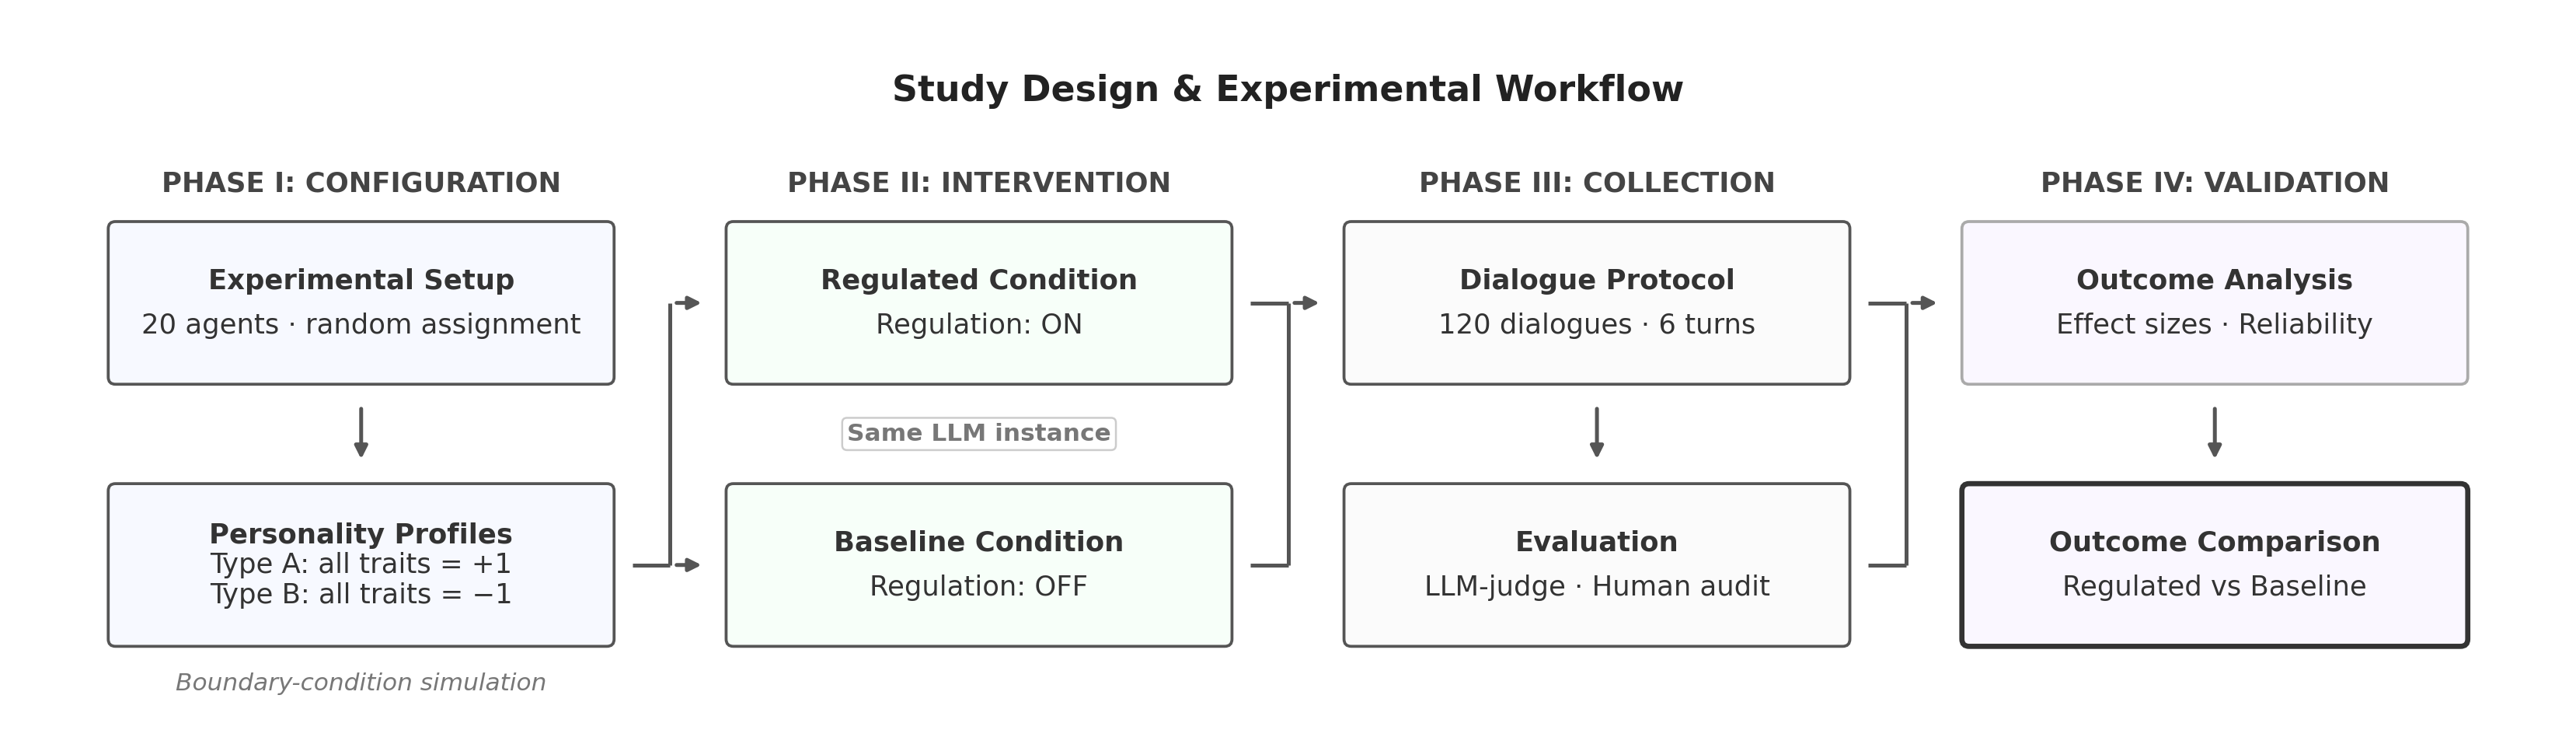
\includegraphics{figures/mdpi/study_design_mdpi.png}
\caption{Study workflow integrating system configuration, dialogue generation, structured LLM-based evaluation (with author-conducted qualitative review), and statistical analysis.}
\label{fig:1}
\end{figure}

\subsubsection{Sample Size Considerations}\label{sample-size-considerations}

The 20 dialogue sessions (5 per cell; 10 per assistant type when aggregated across profiles) represent distinct GPT-4 instantiations with condition-specific system prompts, not human subjects. This sample size was selected for architectural validation purposes based on: (1) a controlled simulation design with limited stochastic variation, (2) computational cost constraints appropriate for proof-of-concept testing, and (3) focus on demonstrating implementation fidelity rather than estimating population-level effects {[}33{]}.

Traditional power analysis is inappropriate because: (1) simulations are controlled and not designed to estimate population-level variability, (2) observed ceiling effects (zero variance) violate power analysis assumptions, and (3) the goal is technical validation, not inferential generalization.

Future human validation will require larger samples (e.g., n $\approx$ 50--100 per condition), in line with clinical trial standards for statistical power, attrition, and inter-individual variability, to capture real-world heterogeneity absent from this simulation {[}34,35,36{]}.

\subsubsection{Ethics and Transparency}\label{ethics-and-transparency}

No human subjects were involved in this study; the user-side prompts/questionnaires were written manually, and the resulting dialogues were generated in a controlled manner using GPT-4-based agents following predefined personality profiles. As the data were synthetic, non-identifiable, and created solely for technical validation, the study fell outside the scope of human-subject research as defined by established ethical frameworks, and formal ethics approval was therefore not required {[}37{]}.

Future studies involving human participants will require full institutional review board approval, comprehensive informed consent addressing AI-based personality profiling and data usage, real-time safety monitoring with clear escalation pathways for psychological distress, and ongoing oversight by qualified mental health professionals {[}38,39{]}. Ethical design of agentic conversational systems should also address questions of interactional respect and user autonomy {[}14{]}.

\subsection{Personality-Adaptive System Architecture}\label{personality-adaptive-system-architecture}

The personality-adaptive system centers on turn-by-turn Big Five detection and regulation over the user model, \textbf{integrated in PROMISE} {[}7{]} through state-attached instructions, storage-backed trait values, and finite-state transitions. Its distinguishing mechanisms are: (i)~\textbf{tri-state personality detection}, with each OCEAN dimension encoded as $\{-1, 0, +1\}$ and an explicit \emph{neutral} state when evidence is insufficient (Table~\ref{tab:1}); (ii)~\textbf{cumulative evidence updating}, so each user turn refines trait estimates from the full dialogue history rather than from isolated utterances; (iii)~\textbf{confidence-threshold triggering}, committing a trait out of neutrality only when detector confidence exceeds $\tau$ (specified in Section~\ref{personality-detection-pipeline}); (iv)~\textbf{parallel per-trait detectors}, i.e., independent LLM-based probes per dimension scored concurrently; and (v)~\textbf{Zurich Model trait-to-behavior mapping}, translating non-neutral traits into stylistic regulation directives along Security, Arousal, and Affiliation before response generation (Section~\ref{theory-driven-regulation}). These mechanisms define the technical contribution evaluated in our simulation; the D--R--E workflow was conceived in prior work {[}68{]} (``a PROMISE-orchestrated pipeline linking per-turn OCEAN detection to Zurich Model-aligned regulation and structured LLM-based evaluation'') and is here extended with a controlled factorial design and systematic statistical outcome analysis.

Within PROMISE, we organize work into Detection (D), Regulation (R), and Evaluation (E) modules for structured operation and quality logging (Figure~\ref{fig:2}); we refer to this three-stage pipeline as the \emph{D--R--E pipeline} throughout the paper. PROMISE supplies model-driven orchestration via hierarchical state-machine modeling. In PROMISE, an interaction is encapsulated as an Agent wrapping a state machine composed of States (with state-specific instruction templates and behaviors) connected by Transitions governed by Decisions (e.g., guards or triggers) and accompanied by Actions (e.g., extraction or summarization). These elements operate over an interaction storage abstraction implemented as a key--value store {[}7{]}. This structure enables explicit state transitions, systematic composition of instructions from modular parts, and transparent logging of decisions and actions across complex interactions.

We embed the core D--R--E pipeline into PROMISE's state-orchestrated architecture as follows:

\begin{itemize}
\item
  \textbf{Detection}: Trait estimation is implemented as a state-driven process that updates a continuous Big Five vector and confidence metrics in the interaction store after each user input. Traits are inferred from linguistic cues in the current interaction context and persist as storage values accessible across states.
\item
  \textbf{Regulation}: Within response-generation states, prompts are augmented with trait-conditioned instructions that softly modulate the assistant's response style---such as tone, pacing, and interpersonal framing---without altering semantic content or task objectives. This is achieved by dynamically composing the base state prompt with trait-aligned augmentation prompts at runtime.
\item
  \textbf{Evaluation}: After each response generation, structured assessment actions execute LLM-based quality checks and log evaluation scores alongside turn identifiers in the interaction store. In the current study, these evaluation outputs are used for offline analysis and do not feed back into detection or regulation during the simulation.
\end{itemize}

This mapping allows the full pipeline to be inspected through PROMISE's explicit state/transition structure and logged decisions/actions, improving reproducibility and auditability of adaptation behavior. The proposed detection--regulation--evaluation logic is conceptually framework-agnostic and could be instantiated in alternative orchestration systems; PROMISE is used here because its declarative state modeling facilitates systematic traceability.

\begin{figure}[H]
\centering
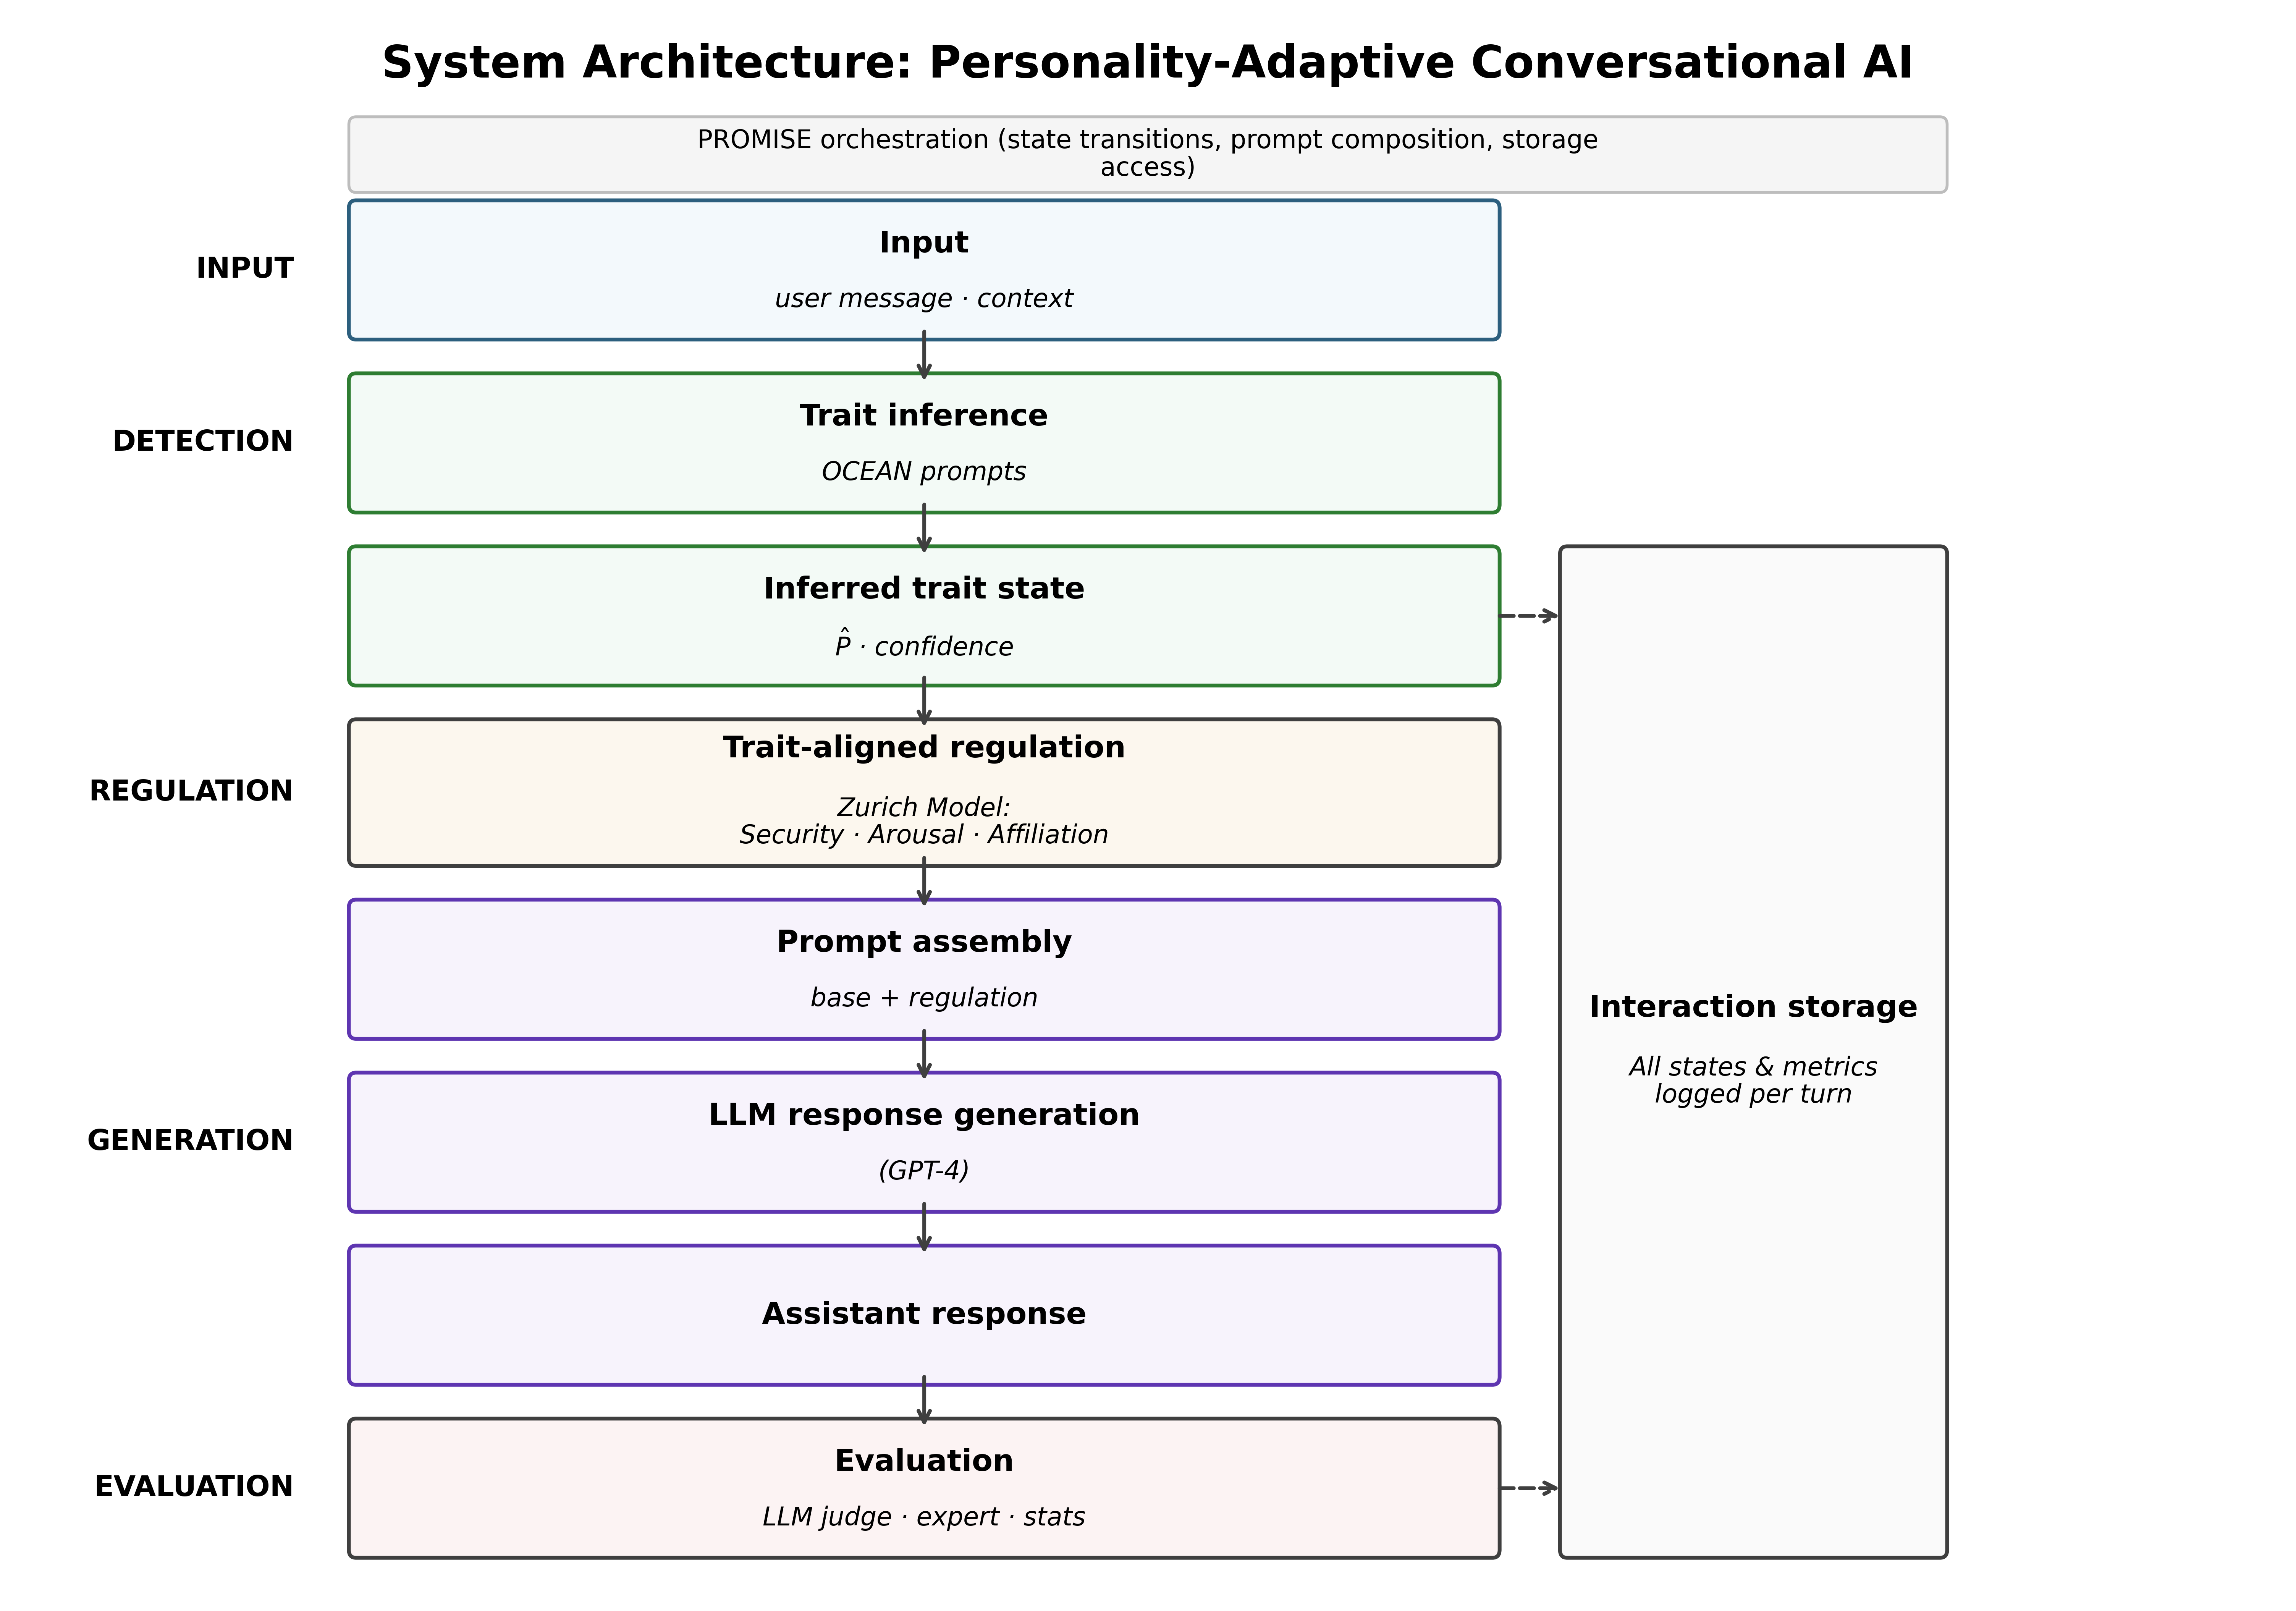
\includegraphics{figures/mdpi/system_architecture_mdpi.png}
\caption{System architecture integrating personality detection (D-module), regulation (R-module), and evaluation (E-module).}
\label{fig:2}
\end{figure}

\subsubsection{Design Principles}\label{design-principles}

The architecture follows three core principles:

\begin{enumerate}
\def\labelenumi{(\roman{enumi})}
\item
  \textbf{Separation of Concerns}: Independent modules with well-defined interfaces enable parallel development and isolated testing. Modules communicate through standardized data structures (JSON) containing personality vectors, regulation instructions, and evaluation scores.
\item
  \textbf{Scalability}: New personality dimensions or regulation strategies can be added without modifying existing components. Trait-to-regulation mapping is externalized as configuration files.
\item
  \textbf{Traceability and Reproducibility}: All detection decisions, regulation instructions, and evaluation scores are logged with timestamps and dialogue turn identifiers. PROMISE's declarative state modeling ensures all behavioral adaptations are traceable to explicit state transitions.
\end{enumerate}

\subsubsection{Data Flow Pipeline}\label{data-flow-pipeline}

The system processes messages through a sequential pipeline (Figure~\ref{fig:3}): (1) User input and dialogue history capture, (2) Personality detection analyzes linguistic cues to infer OCEAN traits, (3) Trait-to-regulation mapping translates personality into behavioral adaptation instructions, (4) Prompt assembly combines regulation with dialogue context, (5) GPT-4 generates personality-adaptive response, (6) Evaluation assesses response quality, and (7) Outputs are logged.

\begin{figure}[H]
\centering
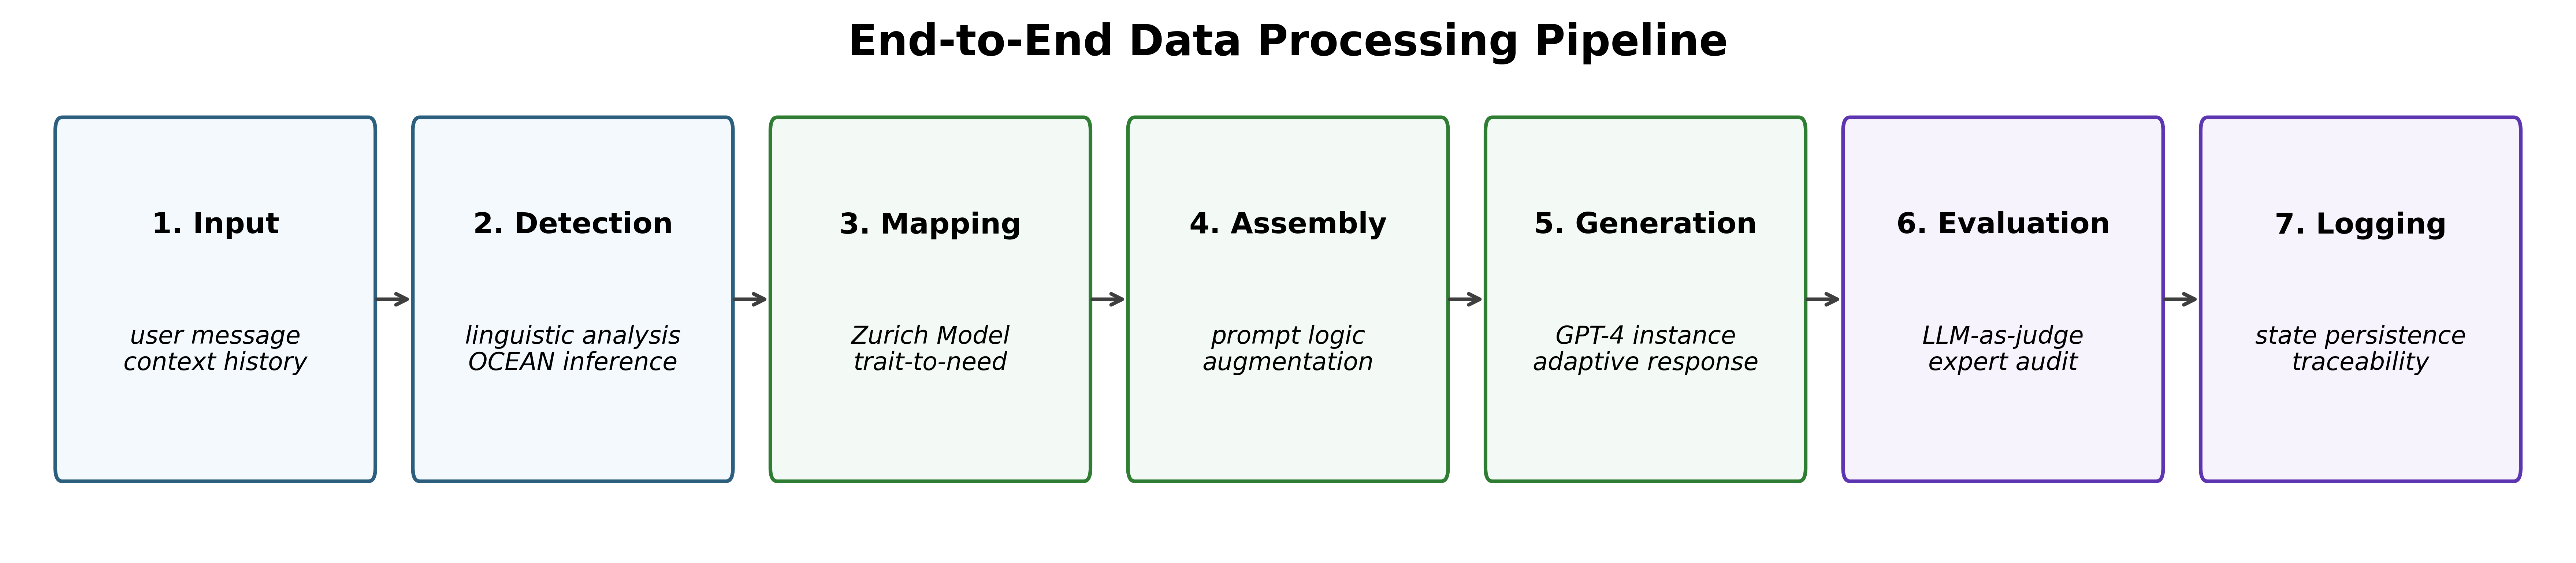
\includegraphics{figures/mdpi/data_flow_mdpi.png}
\caption{End-to-end data flow pipeline.}
\label{fig:3}
\end{figure}

\subsubsection{PROMISE Integration}\label{promise-integration}

PROMISE operationalizes complex interactions by composing prompts from modular parts attached to states and transitions {[}7{]}. In typical PROMISE execution, transition decisions (trigger/guard) are evaluated against the accumulated state utterances before generating the next assistant response; if no transition fires, the assistant response is generated from a composed prompt that includes the state prompt and the dialogue history. PROMISE also supports nested state machines (``outer states'') that maintain an aggregated utterance history across inner states and can inject shared role prompts into all contained states, enabling consistent behavior across multi-stage interactions. Additionally, PROMISE supports placeholder-based instruction templates filled at runtime and actions that extract structured outputs into interaction storage (key--value store), which can be reused by downstream states and system components {[}7{]}. Our integration leverages these mechanisms to (i) persist the current Big Five vector and confidence in storage, (ii) compose trait-aligned regulation instructions into the response-generation prompt, and (iii) log evaluation outputs with turn identifiers for traceability.

\subsection{System Implementation}\label{system-implementation}

This section describes how the system implements (i) real-time personality detection and (ii) theory-driven regulation, both orchestrated within PROMISE (Section~\ref{personality-adaptive-system-architecture}).

\subsubsection{Personality Detection Pipeline}\label{personality-detection-pipeline}

We represent the user's Big Five profile as a five-dimensional vector (P = (O, C, E, A, N)), with each trait ($\in \{-1, 0, +1\}$) {[}3,9,41{]}. In this simulation, the personality vector functions as a predefined reference target for controlled evaluation rather than psychometric ground truth; detection accuracy denotes agreement with the pre-specified simulated profile.

\begin{longtable}[]{@{}
  >{\raggedright\arraybackslash}p{(\linewidth - 4\tabcolsep) * \real{0.2500}}
  >{\raggedright\arraybackslash}p{(\linewidth - 4\tabcolsep) * \real{0.3929}}
  >{\raggedright\arraybackslash}p{(\linewidth - 4\tabcolsep) * \real{0.3571}}@{}}
\caption{Big Five personality trait operationalization. Neuroticism is inverse-coded: +1 denotes emotional stability (low neuroticism), and -1 denotes emotional vulnerability (high neuroticism).}\label{tab:1}\\
\toprule\noalign{}
\begin{minipage}[b]{\linewidth}\raggedright
Trait
\end{minipage} & \begin{minipage}[b]{\linewidth}\raggedright
+1 (High)
\end{minipage} & \begin{minipage}[b]{\linewidth}\raggedright
-1 (Low)
\end{minipage} \\
\midrule\noalign{}
\endhead
\bottomrule\noalign{}
\endlastfoot
Openness & Curious, imaginative, open to novelty & Prefers routine, resistant to new ideas \\
Conscientiousness & Organized, disciplined, structured & Disorganized, impulsive, spontaneous \\
Extraversion & Outgoing, energetic, assertive & Reserved, quiet, withdrawn \\
Agreeableness & Cooperative, empathetic, friendly & Critical, skeptical, confrontational \\
Neuroticism* & Calm, emotionally stable, resilient & Anxious, emotionally sensitive, insecure \\
\end{longtable}

After each user input, the system updates (P) using cumulative evidence across dialogue history, following a belief-updating logic similar to Bayesian belief updating {[}43{]}. PROMISE orchestrates this pipeline via hierarchical state machines, parallel trait detectors, and explicit transition logic (Section~\ref{personality-adaptive-system-architecture}). Inference produces trait values (-1/0/+1) and confidence scores, with trait state transitions triggered when confidence exceeds $\tau$ = 0.7 (Figure~\ref{fig:4}).

\begin{figure}[H]
\centering
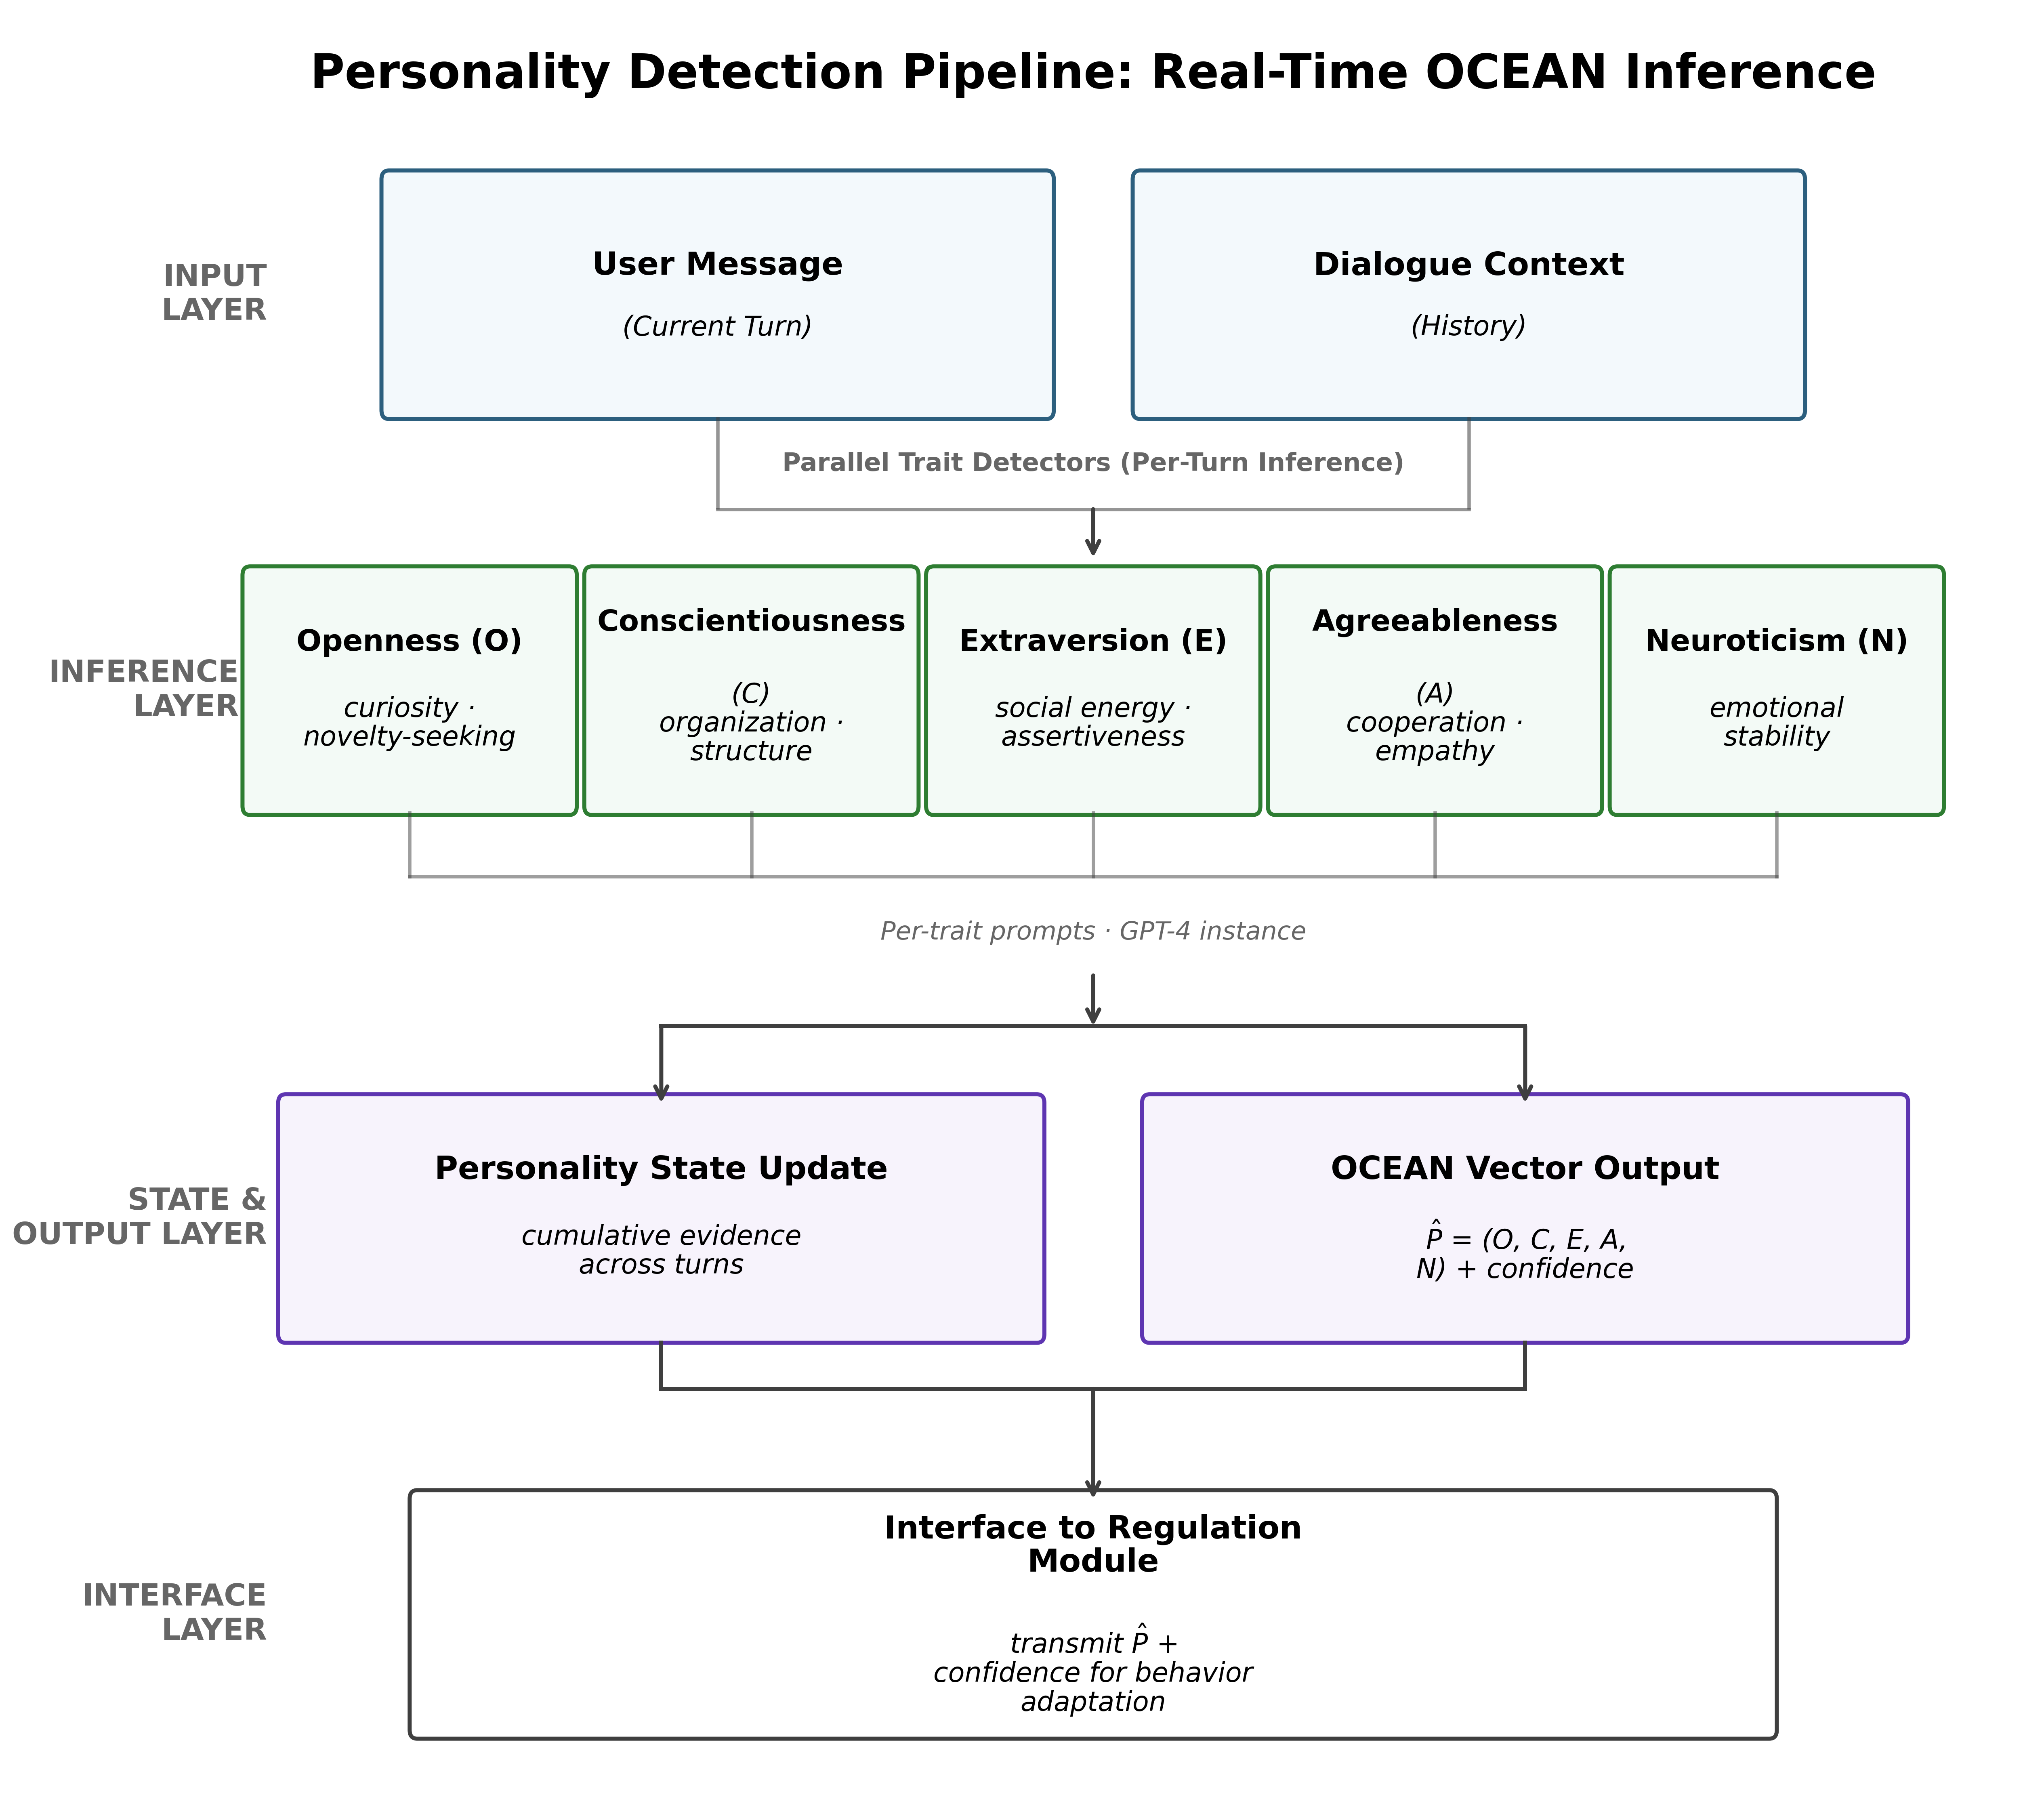
\includegraphics{figures/mdpi/detection_pipeline_mdpi.png}
\caption{Personality detection pipeline implementing turn-by-turn Big Five inference.}
\label{fig:4}
\end{figure}

The detection component is implemented as a modular service integrated into PROMISE. It uses GPT-4 (gpt-4-0613) with trait-specific prompts grounded in personality psychology {[}44--50{]}. The pipeline executes the following stages: (1) message processing, (2) prompt assembly, (3) parallel LLM inference across traits, (4) response parsing and confidence assessment, (5) state update, and (6) downstream transmission to the regulation module.

Average processing time was 2.3 ± 0.8 seconds per turn (measured across 120 turns), with parallel trait detection reducing latency by \textasciitilde60\% versus sequential processing.

\subsubsection{Theory-Driven Regulation}\label{theory-driven-regulation}

Regulation translates detected traits into behavioral adaptations grounded in the Zurich Model of Social Motivation {[}10,26--29{]}, which links personality to three motivational domains: Security, Arousal, and Affiliation (Section~\ref{from-affective-computing-to-personality-aware-digital-support}). Table~\ref{tab:2} and Figure~\ref{fig:5} present the mapping from Big Five traits to motivational domains and corresponding behavioral adjustment strategies.

\begin{figure}[H]
\centering
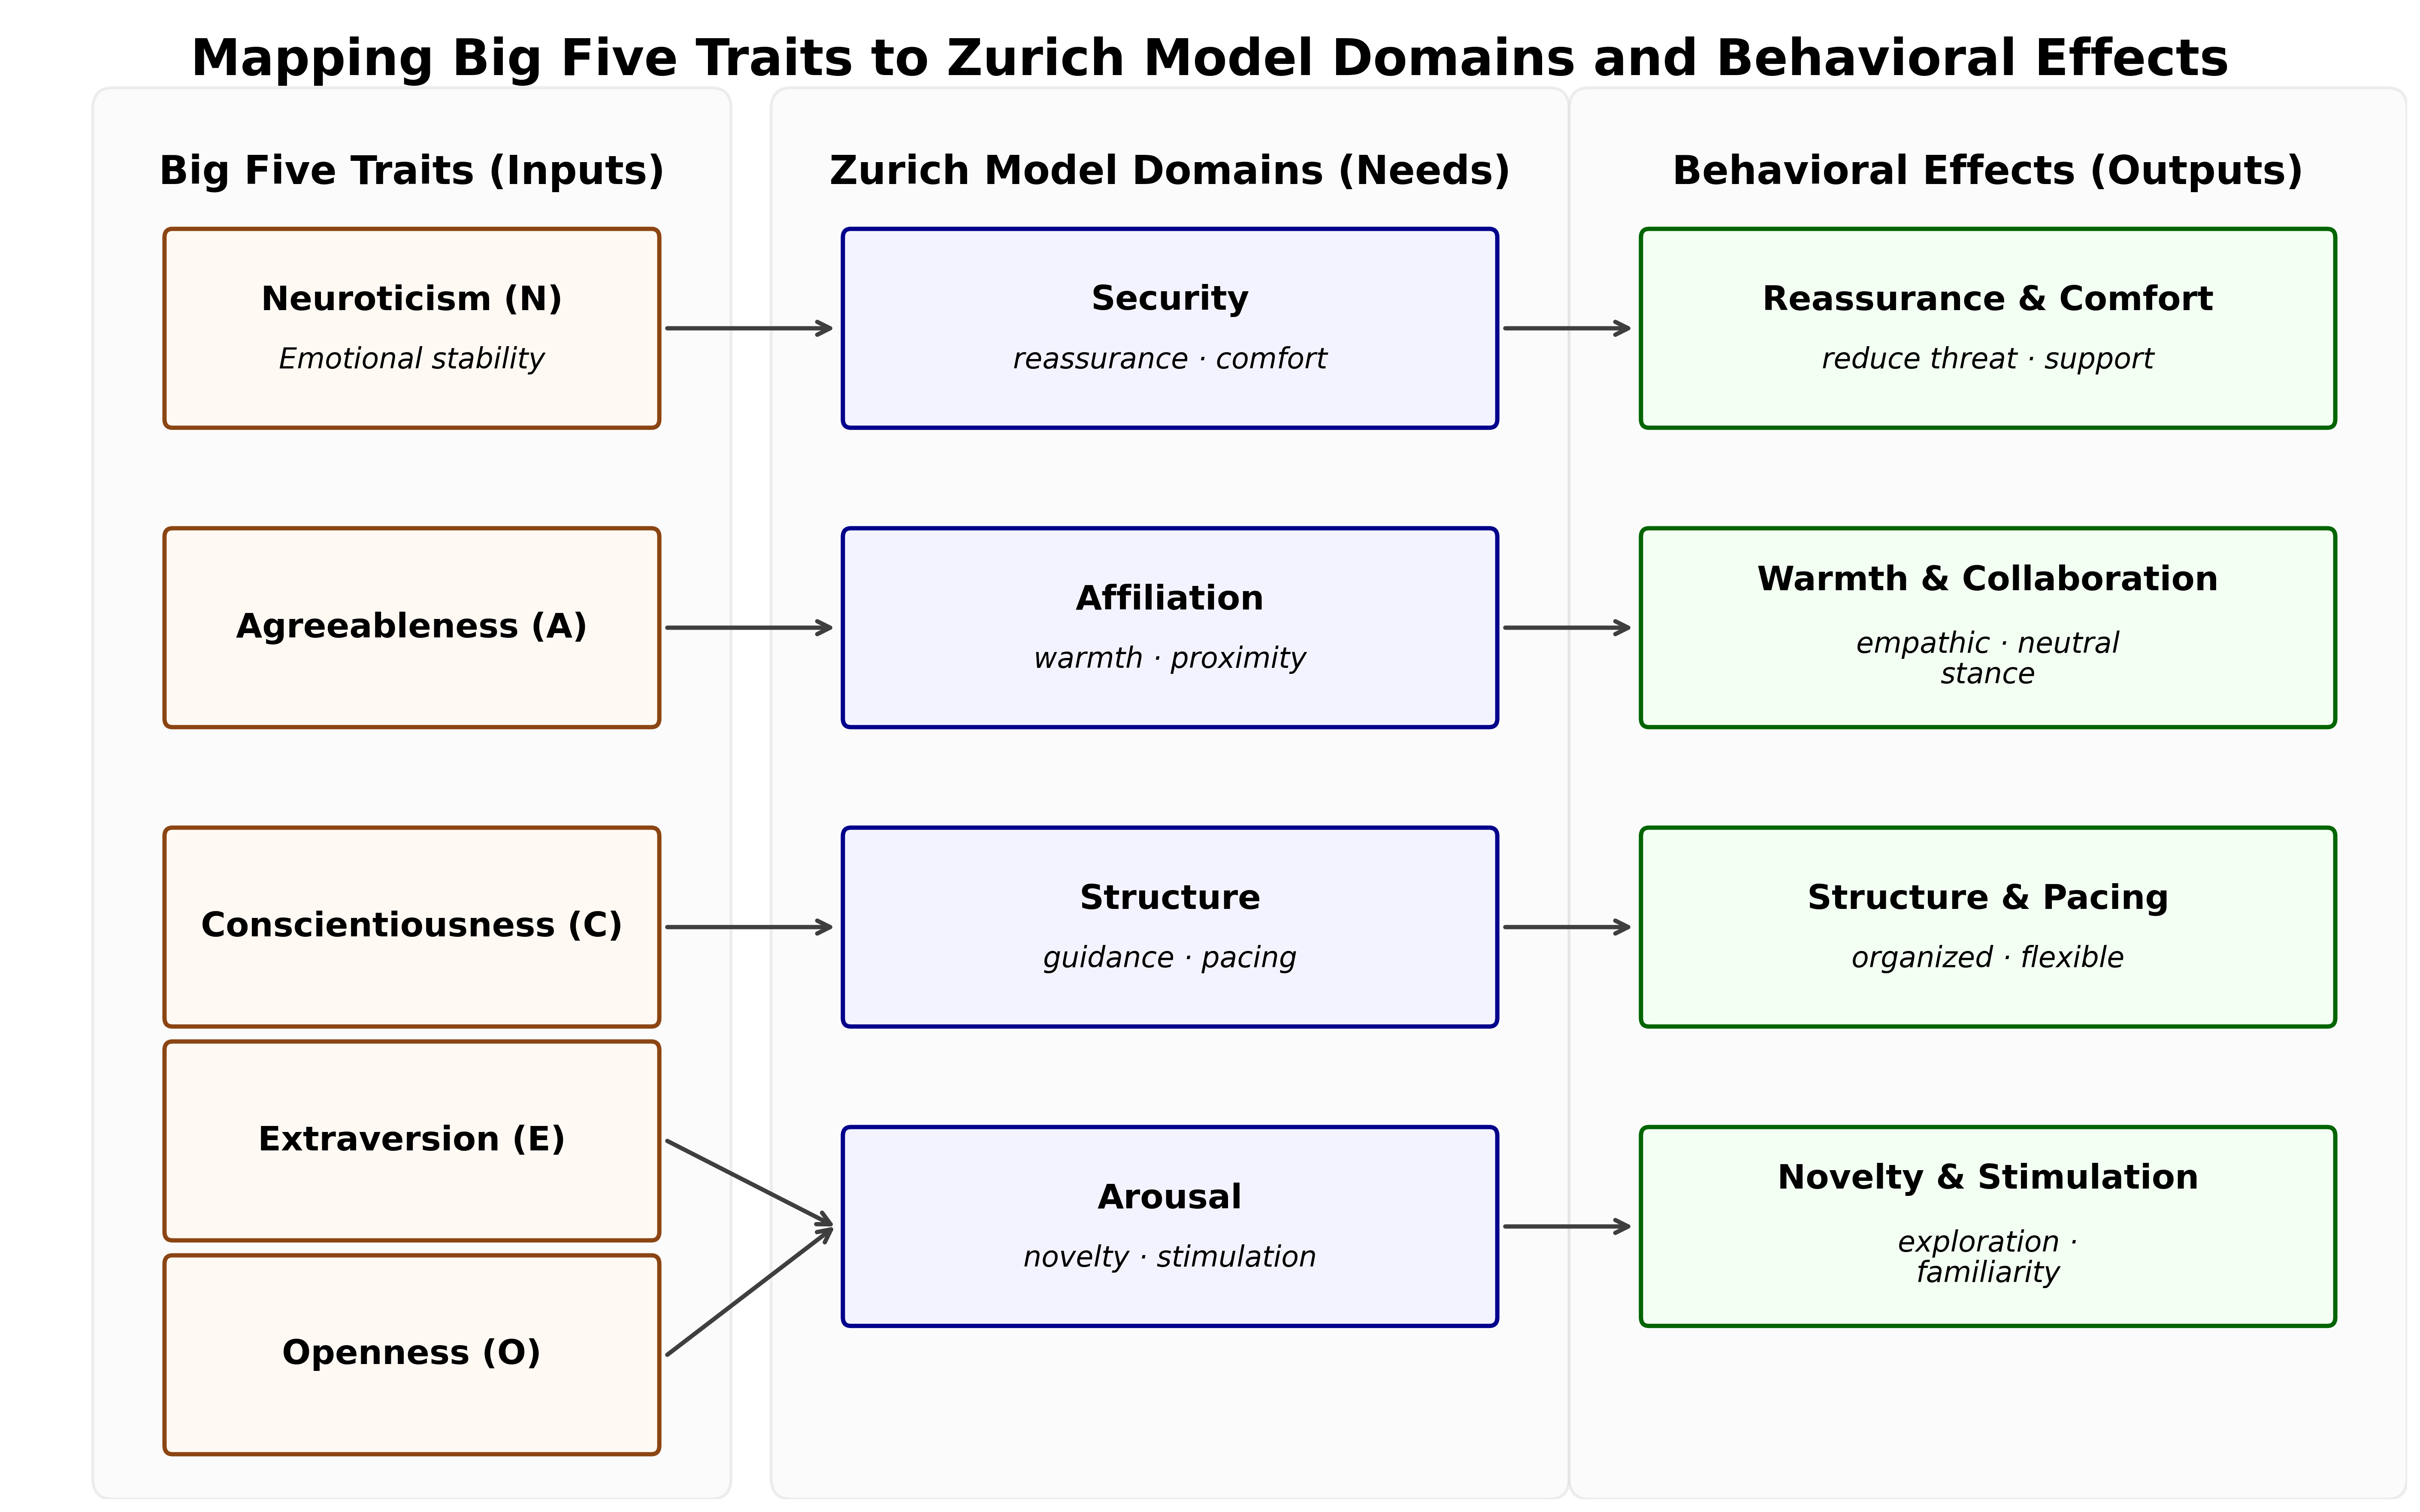
\includegraphics{figures/mdpi/trait_mapping_mdpi.png}
\caption{Mapping from Big Five traits to motivational domains to conversational behavior effects.}
\label{fig:5}
\end{figure}

\begin{longtable}[]{@{}
  >{\raggedright\arraybackslash}p{(\linewidth - 6\tabcolsep) * \real{0.1300}}
  >{\raggedright\arraybackslash}p{(\linewidth - 6\tabcolsep) * \real{0.2600}}
  >{\raggedright\arraybackslash}p{(\linewidth - 6\tabcolsep) * \real{0.3100}}
  >{\raggedright\arraybackslash}p{(\linewidth - 6\tabcolsep) * \real{0.3000}}@{}}
\caption{Behavioral adjustment strategies mapped by Zurich Model motivational domain. Conscientiousness modulates interaction structure independently of the three core domains.}\label{tab:2}\\
\toprule\noalign{}
\begin{minipage}[b]{\linewidth}\raggedright
Domain
\end{minipage} & \begin{minipage}[b]{\linewidth}\raggedright
Trait
\end{minipage} & \begin{minipage}[b]{\linewidth}\raggedright
+1 (High)
\end{minipage} & \begin{minipage}[b]{\linewidth}\raggedright
-1 (Low)
\end{minipage} \\
\midrule\noalign{}
\endhead
\bottomrule\noalign{}
\endlastfoot
Security & Neuroticism (N) & Reassure stability and confidence & Offer extra comfort; acknowledge anxieties \\
Arousal & Openness (O) & Invite exploration and novelty & Focus on familiar topics; reduce novelty \\
Arousal & Extraversion (E) & Energetic, sociable tone & Calm, low-key style with reflective space \\
Affiliation & Agreeableness (A) & Warmth, empathy, collaboration & Neutral, matter-of-fact stance \\
Cross-cutting & Conscientiousness (C) & Provide organized, structured guidance & Flexible, relaxed, spontaneous demeanor \\
\end{longtable}

After each personality update, PROMISE composes an integrated regulation instruction by concatenating trait-relevant behavior prompts for all non-neutral traits (Figure~\ref{fig:6}). When trait recommendations conflict, the system prioritizes emotional safety (Security domain) over stimulation (Arousal domain), consistent with clinical guidance {[}51{]}.

\begin{figure}[H]
\centering
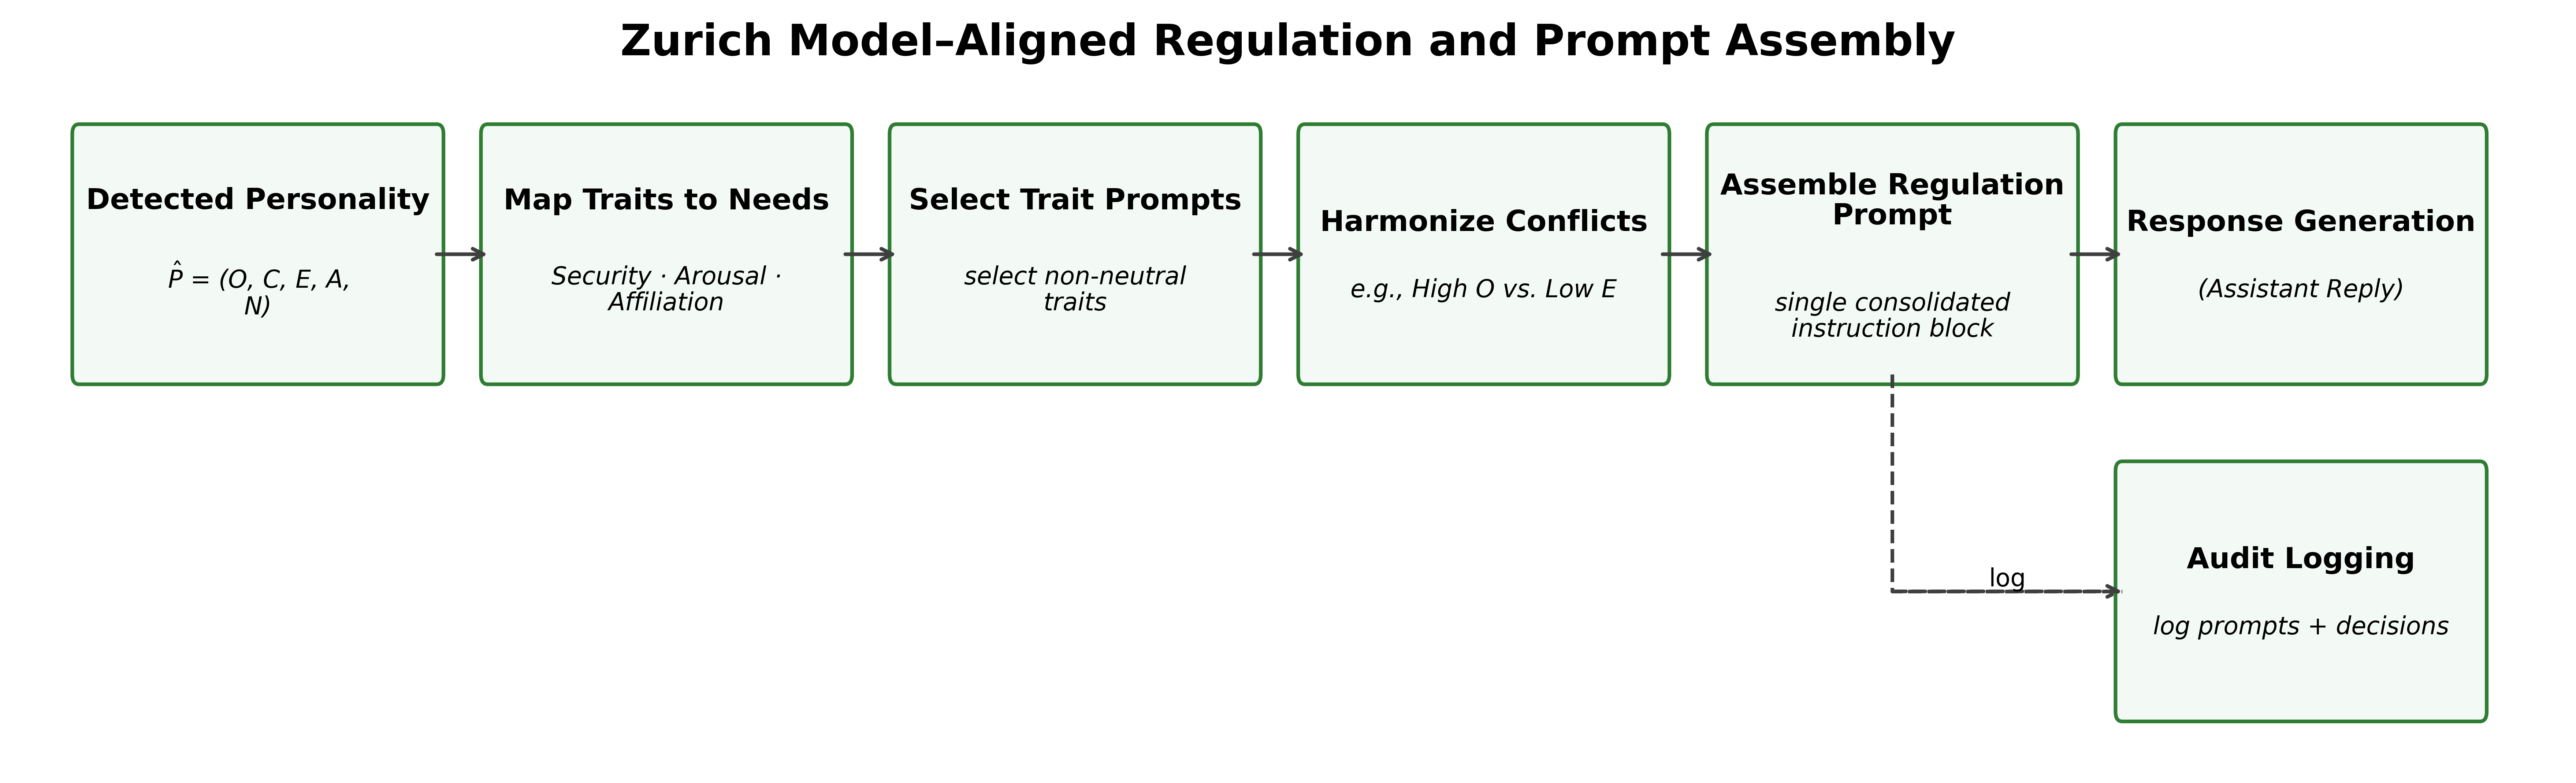
\includegraphics{figures/mdpi/regulation_workflow_mdpi.png}
\caption{Regulation workflow: after each personality update, PROMISE concatenates trait-relevant behavior prompts for all non-neutral traits and assembles an integrated regulation instruction, prioritizing the Security domain over Arousal in cases of conflict.}
\label{fig:6}
\end{figure}

\subsection{Experimental Materials and Procedure}\label{experimental-materials-and-procedure}

\subsubsection{Personality Profile Simulation}\label{personality-profile-simulation}

We implemented two boundary-condition personality profiles representing extremes of human personality variation {[}40,42,53{]}. Type A (all traits: $+1, +1, +1, +1, +1$) embodied extreme positive trait levels. Type B (all traits: $-1, -1, -1, -1, -1$) embodied opposite extremes.

These extreme configurations were deliberately selected to maximize signal for detection and regulation mechanisms. While not representative of typical distributions {[}3{]}, such profiles offer superior diagnostic value for validating this implementation before testing with moderate profiles {[}53{]}.

Detection and regulation performance are evaluated against these synthetic reference profiles as ground truth within the simulation environment. Profiles were encoded into GPT-4 system prompts consistently exhibiting target trait levels across turns.

\subsubsection{Agent Configuration}\label{agent-configuration}

Twenty dialogue sessions (assistant-condition instantiations) were generated across four $2 \times 2$ cells: Regulated--Type~A ($n=5$), Regulated--Type~B ($n=5$), Baseline--Type~A ($n=5$), Baseline--Type~B ($n=5$). Regulated assistants received system prompts incorporating dynamic detection modules and trait-aligned regulation instructions, with inferences updating per-turn. Baseline assistants received static supportive response prompts without personality-specific adaptation. Each assistant instantiation used a separate GPT-4 call configuration (model: gpt-4-0613, temperature=0.7, max\_tokens=500). GPT-4 (gpt-4-0613) was selected because it represented the state-of-the-art instruction-following model at the time of data collection (June--August 2024) and provided the balance of controllability, context length, and response quality required by the PROMISE orchestration framework. The core architectural findings---that explicit regulation instructions produce consistent personality-need fulfillment whereas non-adaptive prompting does not---are expected to generalize to successor models (e.g., GPT-4o, GPT-4-turbo); if anything, stronger base models may yield higher detection accuracy and more nuanced regulation, though independent validation with those models remains necessary.

\subsubsection{Dialogue Structure and Data Collection}\label{dialogue-structure-and-data-collection}

For each personality type (A and B), we generated 5 regulated and 5 baseline dialogue sessions. Each session consisted of 6 user--assistant exchanges (i.e., 6 assistant responses paired with 6 user messages), resulting in 120 assistant turns total across the full design (2 profiles $\times$ 2 assistant types $\times$ 5 sessions $\times$ 6 assistant turns). All conversations followed a standardized six-exchange structure balancing sufficient interaction depth for valid personality detection with manageable evaluation complexity.

Each session followed a consistent scenario progression across the six exchanges (opening support offer $\rightarrow$ initial disclosure $\rightarrow$ elaboration $\rightarrow$ reframing $\rightarrow$ coping/next-step guidance $\rightarrow$ closing), with user messages generated to reflect the target personality profile and assistants responding either with regulated (personality-adaptive) or baseline (non-adaptive) strategies.

User messages were generated by separate GPT-4 instances (model: gpt-4-0613) instantiated with personality profile prompts ensuring consistent trait expression. Conversations were exported into structured Evaluation Matrices (Excel format). Data collection occurred over 4 weeks (June--July 2024). The simulation data were generated during the initial system development phase, prior to the present study {[}68{]}.

\subsection{Evaluation Procedure}\label{evaluation-procedure}

\subsubsection{Evaluation Criteria and Scoring Framework}\label{evaluation-criteria-and-scoring-framework}

The evaluation measured effectiveness of personality-regulated assistant interactions versus baselines using a structured Evaluation Matrix and a dedicated Evaluator GPT, with each assistant output scored on detection accuracy, regulation effectiveness, emotional tone, relevance, and fulfillment of personality-specific emotional needs. The evaluator methodology was conceived in prior work {[}68{]} (``a dedicated GPT-4 evaluator instance scoring regulated turns across five criteria and baseline turns across three criteria on a trinary Yes/Not-Sure/No scale, assessed row-by-row with full dialogue context and personality profile''). Regulated assistants were evaluated across five criteria: Detection Accuracy, Regulation Effectiveness, Emotional Tone Appropriate, Relevance \& Coherence, and Personality Needs Addressed.

Baseline assistants were assessed on three criteria only (Emotional Tone, Relevance \& Coherence, Personality Needs), as detection and regulation were not implemented. All criteria used a trinary scoring scale (\textit{Yes} = 2, \textit{Not Sure} = 1, \textit{No} = 0) {[}54{]}. Figure~\ref{fig:7} illustrates the full evaluation framework and scoring pipeline.

\begin{figure}[H]
\centering
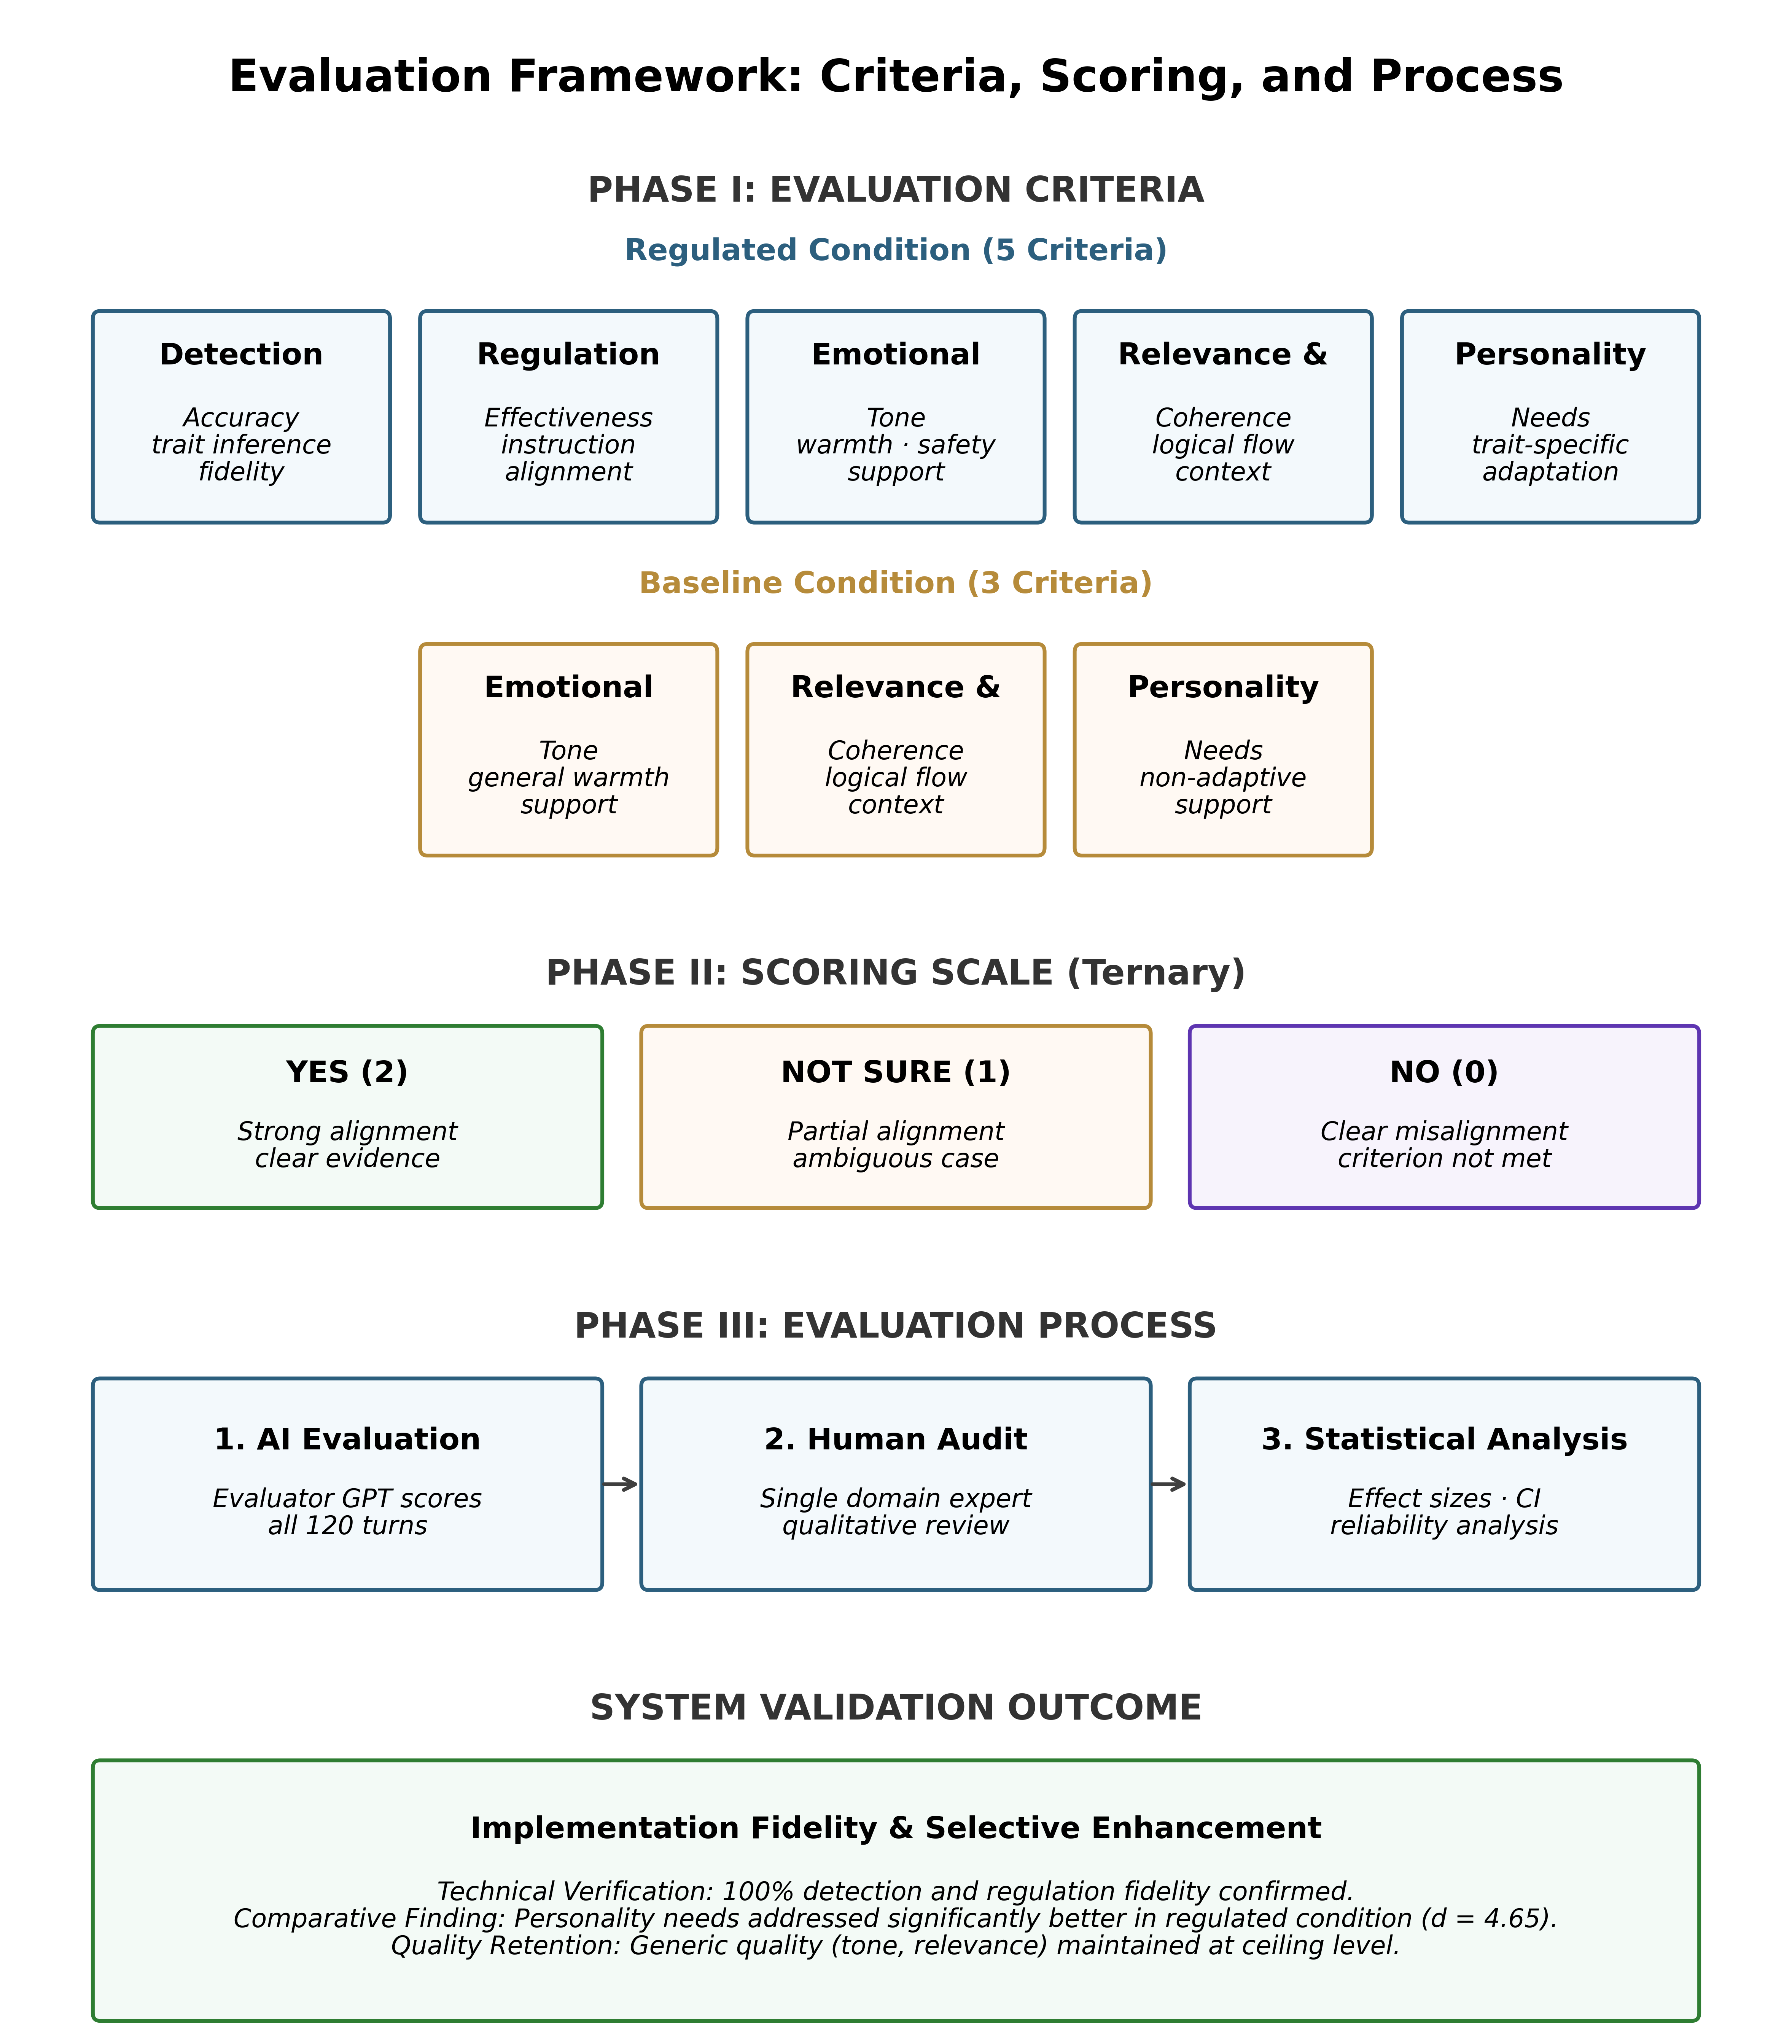
\includegraphics{figures/mdpi/evaluation_framework_mdpi.png}
\caption{Evaluation framework and scoring pipeline.}
\label{fig:7}
\end{figure}

\subsubsection{LLM-Based Evaluator System}\label{llm-based-evaluator-system}

A specialized Evaluator GPT-4 instance was developed using custom-designed prompts for each criterion, following the ``LLM-as-judge'' paradigm {[}55,56{]}. The evaluator assessed responses objectively by analyzing conversations one row at a time. Measures to mitigate evaluator bias: evaluations conducted separately for regulated and baseline assistants; comprehensive context provided including full dialogue history and personality profile; evaluator informed that detection accuracy improves incrementally; temperature set to 0.3 to reduce stochastic variation.

\subsubsection{Evaluation Validity and Author-Led Qualitative Review}\label{evaluation-validity-and-author-validation}

To address ``AI-evaluating-AI'' concerns, two contributing authors (Samuel Devdas and Jiahua Duojie) reviewed all evaluation matrices and provided qualitative commentary for each rated item. Their assessments largely aligned with the agent-generated detections and criterion judgements across the regulated conversations, with one instance marked as uncertain. These author notes provide an internal audit trail supporting the face validity and plausibility of automated ratings; they do \emph{not} constitute impartial verification by independent external raters.

As quantitative ratings are LLM-generated and qualitative validation was performed by study authors, the results should be interpreted as proof-of-concept evidence under controlled simulation conditions, with attendant risk of confirmation bias. This design offers interpretive support rather than quantitative inter-rater reliability or third-party expert certification. Establishing full evaluation credibility requires: (i) at least two independent human raters scoring an overlapping subset of turns to quantify inter-rater reliability (e.g., Krippendorff's $\alpha$ {[}11{]}), and (ii) human--AI agreement analysis for automated scoring (e.g., Cohen's $\kappa$ {[}57,58{]}).

\subsection{Analysis and Reproducibility}\label{analysis-and-reproducibility}

\subsubsection{Primary and Secondary Outcomes}\label{primary-and-secondary-outcomes}

The primary outcome was ``Personality Needs Addressed,'' measured on a trinary scale (\textit{Yes} = 2, \textit{Not Sure} = 1, \textit{No} = 0). Secondary outcomes included Detection Accuracy, Regulation Effectiveness, Emotional Tone Appropriateness, and Relevance \& Coherence. Ratings were applied at the assistant-turn level (10 dialogue sessions per condition $\times$ 6 assistant turns = 60 outputs per condition), yielding 60 observations per metric {[}59{]}.

\subsubsection{Statistical Analysis}\label{statistical-analysis}

Between-group differences were evaluated using two-tailed independent samples \textit{t}-tests for normally distributed metrics and Mann-Whitney U tests for non-normally distributed metrics (normality assessed via Shapiro-Wilk tests, $\alpha$ = 0.05). Effect sizes were calculated using Cohen's d with pooled standard deviation and interpreted using conventional thresholds (small d = 0.2, medium d = 0.5, large d = 0.8) {[}60{]}. For the primary outcome, we also report Cliff's \(\delta\) (probability that a randomly chosen regulated score exceeds a randomly chosen baseline score, rescaled to \([-1,1]\)) as a distribution-free complement when conditions show heavy separation on a discrete scale. Confidence intervals (95\%) were calculated using bias-corrected bootstrap (10,000 iterations) {[}61{]}. Statistical significance was set at $\alpha$ = 0.05. All inferential statistics are reported for comparability with prior conversational AI studies and should not be interpreted as evidence of population-level effects {[}62{]}.

\subsubsection{Reproducibility and Computational Environment}\label{reproducibility-and-computational-environment}

All statistical analyses were conducted in Python 3.9+ using scipy (v1.9.0) for statistical tests, numpy (v1.23.0) for effect size calculations, and matplotlib/seaborn for visualizations. Experiments used GPT-4 API (model: gpt-4-0613, OpenAI Python SDK v1.3.5) with temperature = 0.7 for agent responses and temperature = 0.3 for evaluator responses. All random operations used fixed seed (Python: 42).

Complete implementation code, system prompts, experimental protocols, and conversation transcripts are available at GitHub: \url{https://github.com/SamuelDevdas/socialbehaviourregulation-SD}. The repository includes detection module source code (Java 21), regulation prompt templates (JSON), evaluator GPT system prompts (Markdown), complete conversation transcripts (anonymized CSV, 120 turns), statistical analysis scripts (Python/Jupyter notebooks), and Docker configuration files.

Important limitation: GPT-4 API responses exhibit stochastic variation even at temperature = 0 due to probabilistic sampling {[}63{]}. In this study, the fixed random seed (42) and locked model snapshot (gpt-4-0613) are expected to substantially reduce run-to-run variation, though full determinism cannot be guaranteed by design.

